\section{Network (Jan Müller)}\label{s:network}
\subsection{Overview}
The implemented network stack is organised on a code level according to the OSI reference layer. However, on the running system, only the transport layer is running isolated from the others. An overview over the implementation can be seen in figure \ref{f:network_overview}. The receiving side of the slip protocol, the IP protocol and the transport protocols (UDP, ICMP) are running on the same thread to reduce the overhead introduced by scheduling or the even larger overhead of a call to the RPC system. Another advantage of this system is, that there is less possibility of an internal buffer overflow.\\
For the communication between different network related domains, an internal network messaging protocol (INMP) was implemented. This protocol relies on the underlying RPC/URPC implementation. This allows for multiple user level domains accessing the network, for example the implemented udp\_echo and udp\_terminal domains. There is one master domain called network, which starts the network logic. This process takes the own IP address as input. Currently, it is not possible, to change the IP address after this initial setup. \\
Currently, there are two drawbacks: Because the nameserver is used to connect the network domains and does not support cross core lookups, all network tasks have to run on same core. The other drawback is, that it is not possible to have multiple IP addresses, currently. If one tries to run a second network stack on the other core, the behaviour is not defined as the interrupts are not guaranteed to work as intended anymore.

\begin{figure}
\centering
		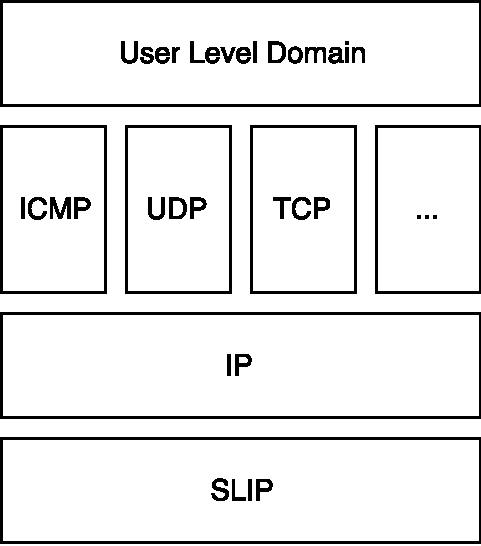
\includegraphics[width=0.2\textwidth]{Images/Network}
		\caption{Code structured according to the OSI reference model.}
\end{figure}

\begin{figure}
\centering
	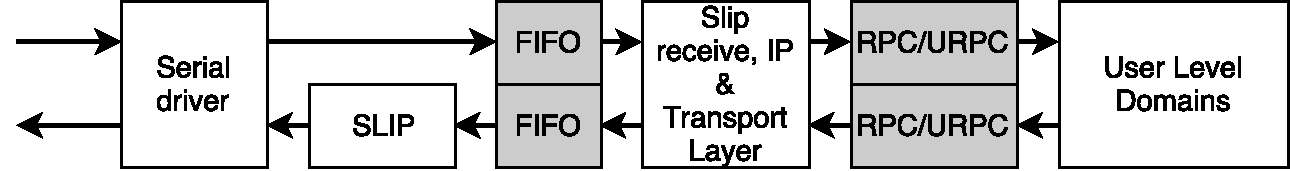
\includegraphics[width=0.9\textwidth]{Images/Packet_flow}
	\caption{The way of a packet from entering on the serial line until leaving the system again. White boxes correspond to individual domains or threads. Gray boxes are used to illustrate the communication channels \label{f:network_overview}}
\end{figure}

\subsection{SLIP}
\subsubsection{Receiving}
The serial input is fed into a circular buffer. A thread implementing the SLIP protocol reads from this buffer byte by byte and does the necessary substitutions given by the protocol. Once the message is complete, it is written into a single packet sized buffer. This might lead to problems if the packets are incoming at a higher rate than they are processed, but this behaviour was not yet encountered and the buffer size could easily be increased.
	The processing should be fast, because it consists only in local comparisons and the reassembly of packet headers for incoming ICMP echo requests. UDP packets are immediately sent to the handler of the corresponding port. A potential overload would show itself in a overflow of the circular buffer which would cause packets to be dropped because of a wrong ip checksum.
\subsubsection{Sending}
When sending, the behaviour is similar. The packet to be sent is read from a small buffer. The substitutions needed for the SLIP protocol are made and the resulting stream of data is written to the serial port byte by byte.
\subsection{IP}
\subsubsection{Receiving}
When the IP handler receives a packet from the SLIP handler, it does some sanity checks first:
\begin{itemize}
	\item Checksum check: check the integrity of the received packet.
	\item Version check: check that the incoming packet is using IPv4.
	\item Length check: make sure that the packet and the header are at least as long as the minimal header length.
	\item Fragmentation check: check for fragmentations (fragmentation flag sequence ID set)
	\item Destination check: check if the device is really the destination of the packet (local IP address matches the destination IP address)
\end{itemize}
If any of these tests fail, the packet is dropped.\\
If the packet passes the tests, the byte order of the source IP address is changed from network byte order to little-endian and is delivered together with the payload to the right protocol. Currently, there are the ICMP and UDP protocols supported. Again, if the packet uses another protocol, the message is dropped.\\
Because the os is not meant to be used as a routing device, the hop count is not reduced or checked on incoming packets.

\subsubsection{Sending}
When the IP handler receives a packet, a standard set of headers are set and the checksum is computed. After the IP packet is arranged, it is handed to the SLIP handler. At the moment, there is no possibility for a domain sending a packet to change the headers of the IP packet (besides the destination address of course). We apply a standard set of headers to all outgoing packets. 

\subsection{ICMP}
The handling of ICMP is simplistic. Currently, the only supported function is the echo reply protocol, which listens to an incoming echo request and replies with a echo reply message. Other incoming ICMP based protocols are dropped.\\
The ICMP handler offers a function which allows any user level domain to send arbitrary ICMP packets. However, there is currently no application making use of this functionality.
\\

\subsection{UDP}
\subsubsection{Open new port}
All UDP ports are implemented by user level domains. A domain can open a new port by sending the appropriate message using the INMP. The domain has to implement the handler for the incoming messages and can then send a request to open a new port to the UDP handler. The handler will check if the port exists and if not, add it to a singly linked list and direct incoming datagrams on that port to the specified domain (again using the internal network message protocol). An open port can be closed again. Currently, there is no check on who is trying to close a port. An obvious improvement would be, to only allow the domain that opened the port and some monitor domain to close the ports. Also, there is currently no check, if the receiving handler of the port is still running or has crashed or exited without closing the port.

\subsubsection{Receiving}
When the UDP handler receives a packet, it UDP handler checks the destination port and forwards the packet to the right user level domain using the INMP. If the port number is not known, the packet is dropped. The incoming and the outgoing port, as well as the source ip address and the payload is sent to the handling domain using the internal network messaging protocol.
\subsubsection{Sending}
Using the internal network messaging protocol, a user level domain can send a packet to the UDP handler which writes the header of the datagram and forwards it to the IP handler. No checksum is created, because according to the RFC on UDP, the UDP checksum is optional.\cite{RFC0768}

\subsection{User Space Applications}
Two user space applications were implemented. An UDP echo server was implemented, that automatically connects to the network process on the same core using the nameserver. All this process does, is to fetch the user input and return it to the user.\\
The UDP terminal server is more interesting. This application is a minimal shell, that allows the user to spawn processes and returns the output of that process to the user. It is currently not allowed to start the TurtleBack shell, as the input integration is not done. The way this works, is that the network terminal app passes a special flag to a spawning process, that signals that it should report to the network terminal. The new process will then use the nameserver to redirect its output to the network terminal. This system could be improved by integrating it to the TurtleBack shell. From a security point of view, a login mechanism should be added.

\subsection{Performance}

\subsubsection{Internal message handling \label{ss:network_internal_message_handling}}
Figure \ref{f:internal_rtt_figure} shows a measurement of the latency of the internal packet handling. For the test, the hardware counter was reset once a packet was completed. The time measurement was taken, before the message was handed back to the serial handler. To get a useful number out of the number of clock cycles, it was divided by the clock frequency of the processor to get the amount of ms passed. The measurement was done once using ICMP packets (figure \ref{f:ping_internal_rtt}) and once using UDP packets (figure \ref{f:udp_internal_rtt}). The values from this measurement steadied on a certain value after one or two measurements. We think, this might be because of allocation of additional ressources, that have to be done when a larger test is run the first tim. \\
We note, that for both protocols, the computation time is linearly increasing with the payload size. We also see, that UDP performes worse than ICMP. This is because there are two extra RPC calls and two context switches more involved in handling these packets.

\subsubsection{Ping \label{ss:network_performance_ping}}
Two tests were performed to measure the performance of the implemented ping-reply mechanism. Both tests consisted of sending pings with 31 different payload sizes. The tests were run 100 times for each size. The Linux ping utility was used to perform both tests.\\
The first test checked the reliability of the system. For a single payload size, we send 100 packets and note, how many replies we receive. The amount of received ping replies is shown in figure \ref{f:ping_yield}. We note, that for sizes that up to about 1.5kB, at least 98\% of the ping packets generate an answer from the system. Note that on sizes larger than 1kB, some of the icmp echo-reply answers contain a faulty payload. This means, that the message sent and received do not have the same payload. However, only less than 3\% of the packets are affected. We see, that there were no replies of the system for payloads larger than 1.5kB. The reason is, that the packets are dropped by the tunsip utility. The error code of -7 indicates a ICMP checksum error. The error happens on the host side, before the packets reach the device under test.\\
In the second test, the actual RTT time for the differently sized ping requests were measured. Sizes larger than 1.5kB were excluded from the test, because of the 0 yield. The mean, as well as the lowest and the highest values for the RTTs can be seen in figure \ref{f:ping_rtt}. Different things can be noted from the data collected: 
\begin{itemize}
	\item The mean RTT is linearly increasing from 0 up to about 800B of payload.
	\item At around 1kB of payload, the system performed the worst. After a peak, the performance gets better again. The cause of this behaviour could not be found.
	\item We note, that the worst case RTT increases for larger payloads
\end{itemize}
The serial connection runs on 115200 Baud. When neglecting the overhead of the slip protocol, this means that we should have a bitrate of about 14kBps. Together with the measurements from \ref{ss:network_internal_message_handling}, we conclude that most of the time that is needed to handle a packet, is needed by the serial connection between the two devices and the interrupt based handling of the incoming and outgoing traffic. 

\begin{figure}
	\begin{subfigure}[c]{0.50\textwidth}
	\centering
		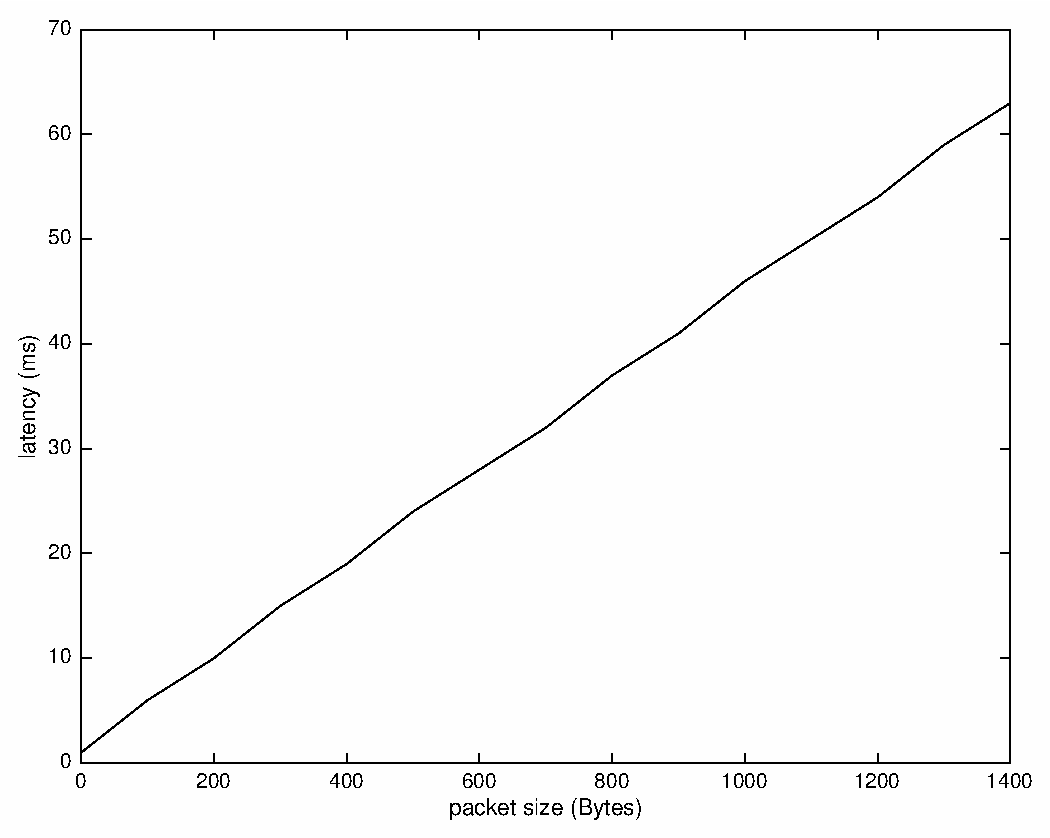
\includegraphics[width=0.9\textwidth]{ping_internal_rtt}
		\subcaption{internal RTT measurement for ICMP \label{f:ping_internal_rtt}}
	\end{subfigure}
\begin{subfigure}[c]{0.50\textwidth}
\centering
		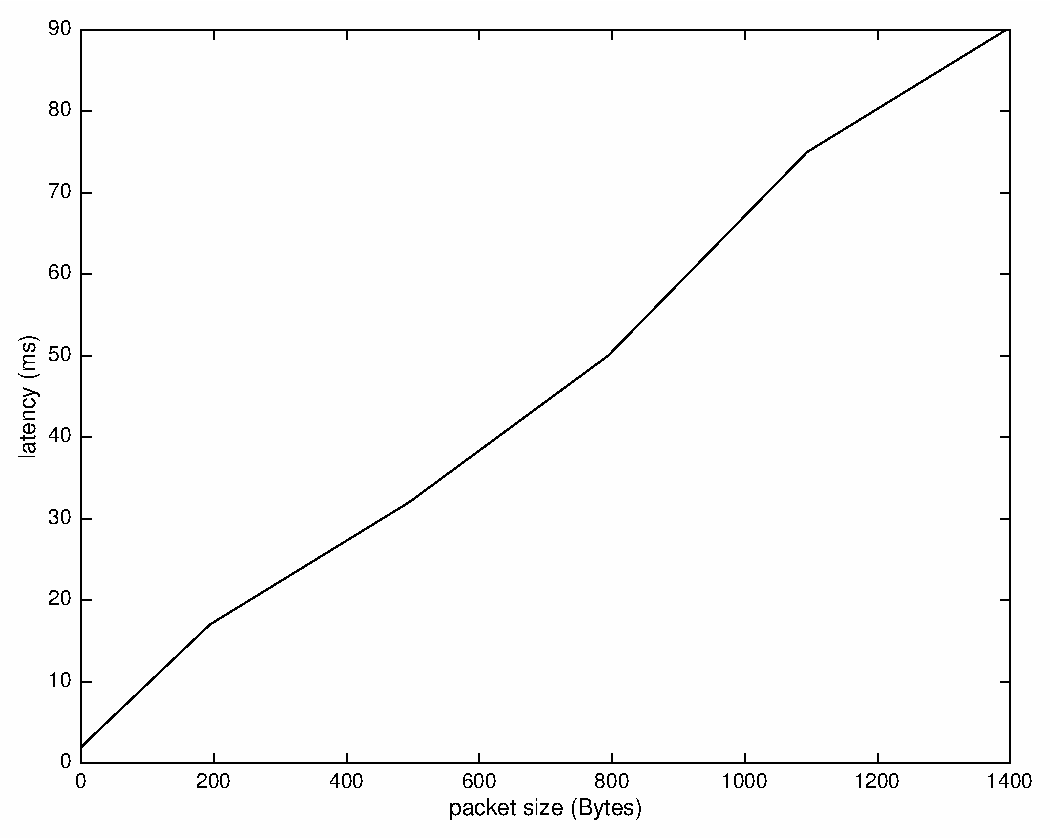
\includegraphics[width=0.9\textwidth]{udp_internal_rtt}
		\subcaption{internal RTT measurement for ICMP \label{f:udp_internal_rtt}}
	\end{subfigure}
	\caption{Latency between completion of packet from serial and handing over of packet to serial}
	\label{f:internal_rtt_figure}
\end{figure}

\begin{figure}
	\begin{subfigure}[c]{0.50\textwidth}
	\centering
		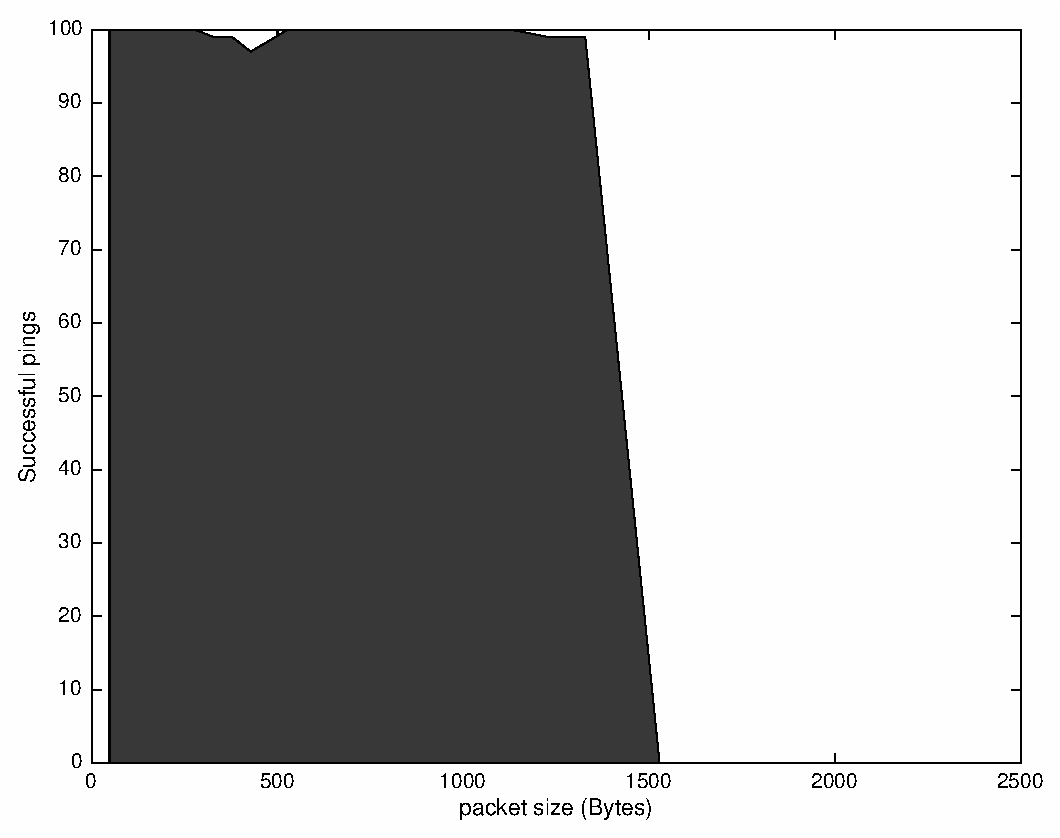
\includegraphics[width=0.9\textwidth]{ping_yield}
		\subcaption{Successful pings (out of 100) for different ping payloads \label{f:ping_yield}}
	\end{subfigure}
\begin{subfigure}[c]{0.50\textwidth}
\centering
		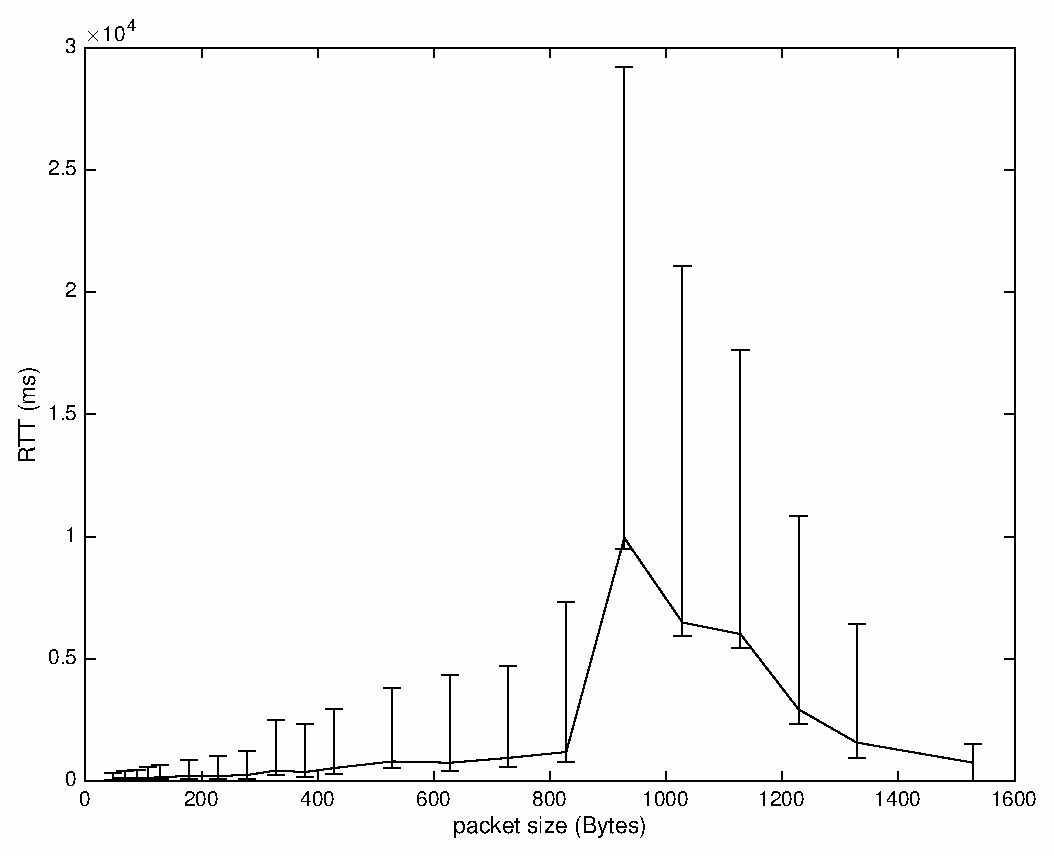
\includegraphics[width=0.9\textwidth]{ping_rtt}
		\subcaption{Round-trip Time (RTT) for different ping payloads \label{f:ping_rtt}}
	\end{subfigure}
	\caption{Ping tests performed using 31 different sized ping request packets.}
	\label{f:ping_figure}
\end{figure}

\subsubsection{UDP echo}
Using nmap, the latency of the response of the echo server was measured. The test was repeated 1000 times. The following values were measured:\\
maximum latency: 230 ms\\
minimum latency: 47 ms\\
mean latency: 68.5 ms\\
the measured values had a standard deviation of 21.7 ms.
Similar statements on the performance as in section \ref{ss:network_performance_ping} can be made.


